\documentclass{myclass}

\begin{document}

\section{What is a neural network?}

History of neural networks dates back at least to the 1950s when F. Rosenblatt proposed the
perceptron model. The basic computational unit in such a network was the McCulloch--Pitts neuron
which realized the following mapping \(\Rbb^n \mapsto \Rbb\)
\[
\boxed
{
   f(\bm{x}) = \varphi \left( \bm{x} \bm{w}^\tpose + b \right)
}
\]
where \(\bm{x} = \mqty[x_1 & \ldots & x_n]\) is the vector of input signals, \(\varphi\) is some
nonlinear activation function and \(\bm{w}\), \(b\) are some parameters (\(\bm{w}\) called the
weights and \(b\) called the bias). Multilayer perceptron was built from many such neurons connected
in layers so that the connections existed only between the neurons in neighboring layers and there
were no connections between the neurons in the same layer. 

\begin{figure}[ht]
   \centering
   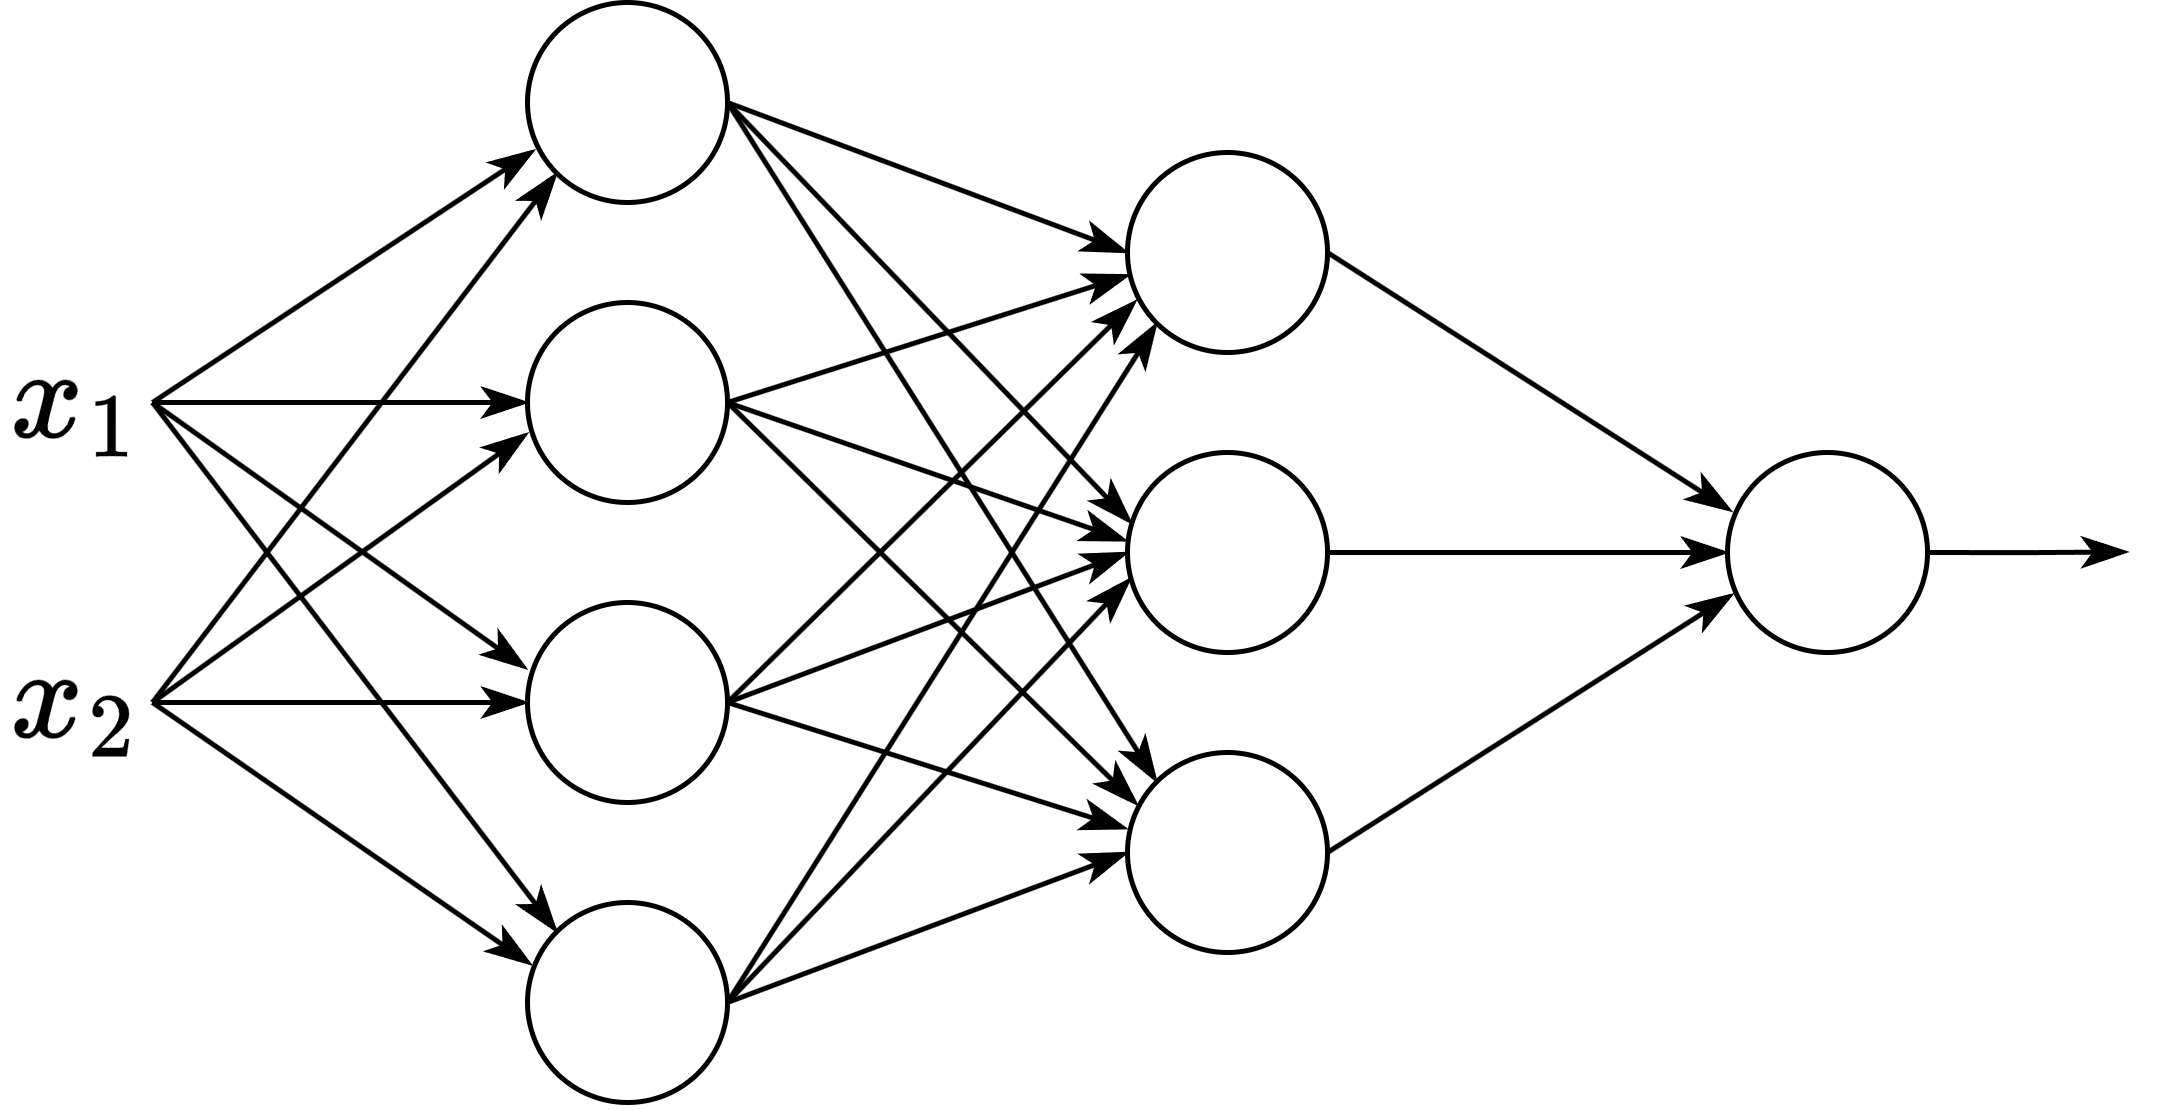
\includegraphics[width=0.85\columnwidth]{figs/nn.png}
\end{figure}

In general neural network is any Directed Acyclic Graph (DAG) in which every vertex \(i\) has the
following attributes.

\medskip

1. Set of previous vertices -- \(\mathscr{P}_i\).

\medskip

2. Set of next vertices -- \(\mathscr{N}_i\).

\medskip

3. Parametrized tensor function \(\bm{F}^{(i)}\) of the form
\[
   \Rbb^{\left(n_{1}^{(1)}, \ldots, n_{k_1}^{(1)}\right)} \times \ldots \times  \Rbb^{\left(n_{1}^{(p)}, \ldots, n_{k_p}^{(p)}\right)} \times \Theta \mapsto \Rbb^{(m_1, \ldots, m_l)}
\]
The function takes \(p\) tensor arguments of dimensions \(k_1,\ldots,k_p\) respectively (input
tensor \(q\) of dimension \(k_q\) has \(n_{r}^{(q)}\) elements along the \(r\) axis) and parameters
\(\bm{\theta}^{(i)} \in \Theta\) and returns a tensor of dimension \(l\). Obviously it must satisfy
\(p = |\mathscr{P}_i|\) and the tensors returned by the parent nodes must have appropriate shapes.

\medskip

4. The gradient functions of the function \(\bm{F}^{(i)}\) w.r.t. to the parameters and w.r.t. all
the inputs, that is for all \(j \in \mathscr{P}_i\) we have the gradient functions
\[
   \pdv{F_\beta ^{(i)}}{\theta_\alpha ^{(i)}}\,,\quad \pdv{F_\beta ^{(i)}}{F_\alpha ^{(j)}} \,,
\]
where \(\alpha\), \(\beta\) are the suitable multi-indices.


\section{Loss functions}

Training of a neural network consists of changing the parameters \(\bm{\theta}^{(i)}\) of the nodes
in such a way as to make the network perform the given task. The task is specified by a training set
\(\mc{X}\) which contains the ''blueprint answers'' of the network. To train the network we
introduce the quantitative measure of networks performance on the dataset which implicitly (through
the outputs of the network) depends on the parameters of the network (here collectively denoted by
\(\bm{\theta}\)) \(L(\mc{X}, \bm{\theta})\). Training can be then phrased as an optimization problem
of the form
\[
   \bm{\theta}^* = \arg \min_{\bm{\theta}} L(\mc{X}, \bm{\theta})
\]
for a fixed training set \(\mc{X}\).

\medskip

There is no single established way of constructing loss functions. One of the more motivated
approaches is based on the maximum likelihood criterion. The idea is that we model our data using
some parametrized statistical model and express the parameters of this model as an output of a
neural network. The loss function is then taken to be the \emph{negated log-likelihood function}. In
this manner one can derive the most common loss functions.


\subsection{Mean Squared Error}

\[
\boxed{ L(\mc{X}, \bm{\theta}) = \frac{1}{2n} \sum_\alpha \left[ y_\alpha - \Phi_\alpha(\bm{X};\bm{\theta}) \right]^2}
\] 
where \(\bm{X}\) is a tensor which can be interpreted as a stack of \(n\) 1-D feature-vectors
residing in the last dimension of \(\bm{X}\), \(\bm{y}\) is the corresponding tensor of \(n\) scalar
continuous outputs for each feature-vector (so called target) and \(\bm{\Phi}\) denotes the neural
network. We also show the derivation of the gradient of the loss function w.r.t. \(\bm{\Phi}\)
\[
\begin{split}
   \pdv{L}{\Phi_\beta} &= \frac{1}{2n} \sum_\alpha 2 \left( \Phi_\alpha - y_\alpha \right) \pdv{\Phi_\alpha}{\Phi_\beta} \\
                       &= \frac{1}{n} \sum_\alpha \left( \Phi_\alpha - y_\alpha \right) \delta_{\alpha\beta}\\
                       &= \frac{1}{n} \left( \Phi_\beta - y_\beta \right)
\end{split}
\]
so finally
\[
\boxed{\pdv{L}{\Phi_\beta} = \frac{1}{n} \left( \Phi_\beta - y_\beta \right) }
\]


\subsection{(Binary) Cross Entropy}

\[
\boxed{
\begin{split} 
   & L(\mc{X}, \bm{\theta}) = -\frac{1}{n} \sum_{\alpha} \left[ t_\alpha \log\pi_\alpha + (1-t_\alpha)\log(1-\pi_\alpha) \right] \\
   & \bm{\pi} = \sigma\left( \bm{\Phi}(\bm{X}; \bm{\theta})\right)\,,\quad \sigma(z) = \frac{1}{1 + \e^{-z}}\,,
\end{split}
}
\] 
where \(\bm{X}\) is a tensor which can be interpreted as a stack of \(n\) 1-D feature-vectors
residing in the last dimension of \(\bm{X}\), \(\bm{t}\) is the corresponding tensor of \(n\) binary
(i.e. 0 or 1) values denoting the class for each feature-vector, \(\sigma\) is the logistic
function, \(\bm{\Phi}\) denotes the neural network and \(\bm{\pi}\) is a tensor of the same shape as
\(\bm{t}\) which contains the probabilities of the positive class.  We also show the derivation of
the gradient of the loss function w.r.t. \(\bm{\Phi}\)
\[
\begin{split}
   \pdv{L}{\Phi_\beta} &= \sum_{\mu} \pdv{L}{\pi_{\mu}} \pdv{\pi_{\mu}}{\Phi_\beta} \\
                       &= \frac{1}{n}\sum_{\mu} \left( \frac{1-t_\mu}{1 - \pi_\mu} - \frac{t_{\mu}}{\pi_{\mu}} \right) \sigma'(\Phi_\mu) \delta_{\mu\beta} \\
                       &= \frac{1}{n} \left( \frac{1-t_\beta}{1 - \pi_\beta} - \frac{t_{\beta}}{\pi_{\beta}}\right) \sigma'(\Phi_\beta)\quad.
\end{split}
\]
Note however that
\[
   \dv{\sigma}{z} = \sigma(z)\left(1 - \sigma(z)\right)\,,
\]
therefore \(\sigma'(\Phi_\beta) = \pi_\beta (1 - \pi_\beta)\) and thus
\[
\boxed{\pdv{L}{\Phi_\beta} = \frac{1}{n}(\pi_\beta - t_\beta)}
\]


\subsection{Cross Entropy}

\[
\boxed
{
\begin{split}
   & L(\mc{X}, \bm{\theta}) = -\frac{1}{n}\sum_{\alpha}\sum_{\beta} t_{\alpha\beta} \log \pi_{\alpha\beta}\\
   & \bm{\pi} = \bm{\sigma}\left( \bm{\Phi}(\bm{X};\bm{\theta}) \right)\,,\quad \sigma_{\alpha'\alpha}(\bm{z}) = \frac{\exp z_{\alpha'\alpha}}{\sum_{\beta} \exp z_{\alpha'\beta}}
\end{split}
}
\] 
where \(\bm{X}\) is a tensor which can be interpreted as a stack of \(n\) 1-D feature-vectors
residing in the last dimension of \(\bm{X}\), \(\bm{t}\) is the corresponding tensor which can be
interpreted as a stack of \(n\) 1-D one-hot-vectors residing in the last dimension of \(\bm{t}\)
encoding the correct class, \(\bm{\sigma}\) is the soft-max function which given the stack of 1-D
vectors independently normalizes each of them so that the entries are non-negative and sum to 1 and
\(\bm{\Phi}\) denotes the neural network. We also show the derivation of the gradient of the loss
function w.r.t~\(\bm{\Phi}\)
\[
   \pdv{L}{\Phi_{\mu\nu}} = \sum_{\mu'\nu'} \pdv{L}{\pi_{\mu'\nu'}} \pdv{\pi_{\mu'\nu'}}{\Phi_{\mu\nu}} = -\frac{1}{n}\sum_{\mu'\nu'} \frac{t_{\mu'\nu'}}{\pi_{\mu'\nu'}} \pdv{\pi_{\mu'\nu'}}{\Phi_{\mu\nu}}\,.
\]
It can easily be shown that
\[
   \pdv{\pi_{\mu'\nu'}}{\Phi_{\mu\nu}} = \delta_{\mu'\mu} \delta_{\nu'\nu} \pi_{\mu'\nu'} - \delta_{\mu'\mu} \pi_{\mu'\nu'} \pi_{\mu' \nu}
\]
and thus
\[
   \pdv{L}{\Phi_{\mu\nu}} = -\frac{1}{n} \left( t_{\mu\nu} - \pi_{\mu\nu} \sum_{\nu'} t_{\mu\nu'} \right)\,.
\]
However from the definition of \(\bm{t}\) we have \(\sum_{\nu'} t_{\mu\nu'} = 1\) and thus finally
\[
\boxed{\pdv{L}{\Phi_{\mu\nu}} = \frac{1}{n} \left( \pi_{\mu\nu} - t_{\mu\nu} \right)}
\]

\section{Forward propagation}

Let \(\bm{v}^{(i)}\) be the (tensor) value of the function \(\bm{F}^{(i)}\). To propagate the
(tensor) inputs to the network and get the output we use the following recursive equation
\[
\boxed{ \bm{v}^{(i)} = \bm{F}^{(i)} \left[ \left(\bm{v}^{(j)}\right)_{j \in \mathscr{P}_i} ; \bm{\theta}^{(i)} \right] }'
\] 
and visit the nodes in the \emph{topological order} as this guarantees that we visit every node
exactly once. We assume here that nodes \(\bm{v}^{(i)}\) such that \(\mathscr{P}_i = \varnothing\)
are the inputs to the network and nodes \(\bm{v}^{(i)}\) such that \(\mathscr{N}_i = \varnothing\)
are the output of the network.


\section{Backward propagation}

Let \(L\) be the loss function. In order to compute the derivatives
\(\partial_{\bm{\theta}^{(i)}}L\) we use the following recursive equations
\[
\boxed{
\begin{split} 
   &\pdv{L}{\theta^{(i)}_\alpha} = \sum_\beta \pdv{L}{F^{(i)}_\beta} \pdv{F^{(i)}_\beta}{\theta^{(i)}_\alpha} \\
   &\pdv{L}{F_\alpha^{(i)}} = \sum_{j \in \mathscr{N}_i} \sum_\beta \pdv{L}{F_\beta^{(j)}} \pdv{F_\beta ^{(j)}}{F_\alpha^{(i)}}
\end{split}
}
\] 
where \(\alpha\), \(\beta\) are the suitable multi-indices. We visit nodes in the \emph{reversed
topological order} and compute and store the values of loss function derivatives. All derivatives
are computed for the current values of \(\bm{v}^{(i)}\) and \(\bm{\theta}^{(i)}\), therefore before
backward propagation one must perform forward propagation to compute values \(\bm{v}^{(i)}\).


\section{Stochastic Gradient Descent}

The standard optimization method used to train neural networks is the Stochastic Gradient Descent,
which is an iterative, gradient-based algorithm in which in every step \(t\) we update the
parameters \(\bm{\theta}\) utilizing the gradient information. Let \(\bm{\theta}_t\) denote the
value of parameters \(\bm{\theta}\) at step \(t\) and let \(\bm{v}_t\) be the values of the
functions \(\bm{F}\) at step \(t\). In each step we take a batch \(\mc{X}\)  of training data,
perform forward propagation to compute values \(\bm{v}_t\) and the value of the loss function
\(L(\mc{X},\bm{\theta}_t)\), next perform backward propagation to compute the values of gradients
\((\partial_{\bm{\theta}}L)\left(\mc{X},\bm{\theta}_t\right)\) and
afterwards we update the parameters according to
\[
   \boxed{ \bm{\theta}_{t+1} = \bm{\theta}_t - \eta \pdv{L}{\bm{\theta}}\bigg|_{\bm{\theta}=\bm{\theta}_t} }
\] 
where \(\eta\) is the learning rate.


\subsection{Momentum}

The problem with vanilla SGD is that it gets stuck in the local minima. To overcome this problem one
can take inspiration from simple physics. We first introduce velocity tensor \(\bm{V}\) with the
following update rule
\[
\boxed
{
   \bm{V}_{t+1} = \mu \bm{V}_{t} - \eta \pdv{L}{\bm{\theta}}\bigg|_{\bm{\theta}=\bm{\theta}_t}
}
\] 
where \(0 < \mu < 1\) is the so called \emph{momentum term} and update parameters using
\[
\boxed
{ 
   \bm{\theta}_{t+1} = \bm{\theta}_t + \bm{V}_{t+1}
}
\]


\subsection{Nesterov's Accelerated Gradient}

A simple modification of classical momentum, which (at least theoretically, for convex functions)
improves the convergence rate of the SGD algorithm is the following. Whereas classical momentum
updates the velocities according to
\[
   \bm{V}_{t+1} = \mu \bm{V}_{t} - \eta \pdv{L}{\bm{\theta}}\bigg|_{\bm{\theta} = \bm{\theta}_t}
\]
the Nesterov method uses
\[
\boxed
{
   \bm{V}_{t+1} = \mu \bm{V}_{t} - \eta \pdv{L}{\bm{\theta}}\bigg|_{\bm{\theta} = \bm{\theta}_t + \mu \bm{V}_t}
}
\]
Using the equation above in the way it was written creates certain problems -- the problem is that
the parameters $\bm{\theta}$ we keep in the layers are not the ones we need to compute forward and
backward passes. A simple solution of this complication is to use parameters $\bm{\phi}_t =
\bm{\theta}_t + \mu \bm{V}_t$ instead of $\bm{\theta}_t$ since assuming the same initialization,
$\bm{V}_0 = 0$ and $\bm{V}_{T} \approx 0$ (where $T$ is the number of training epochs) the values of
both parameters coincide and the update equations (\emph{\mbox{Bengio's} equations}) for $\bm{V}_t$
and $\bm{\phi}_t$ have a very simple form
\[
\boxed
{
\begin{split}
   &\bm{V}_{t+1} = \mu \bm{V}_t - \eta \pdv{L}{\bm{\theta}}\bigg|_{\bm{\theta} = \bm{\phi}_t}\\
   &\bm{\phi}_{t+1} = \bm{\phi}_t + \mu^2 \bm{V}_t - \eta (1 + \mu) \pdv{L}{\bm{\theta}}\bigg|_{\bm{\theta} = \bm{\phi}_t}
\end{split}
}
\]


\subsection{Adaptive Moment Estimation (Adam)}

Another problem with vanilla SGD is that it uses the same learning rate for every scalar parameter.
Adam algorithm solves this problem by introducing running averages with exponential forgetting of
both the gradients and the second moments of the gradients.
\[
\boxed{
\begin{split} 
   &\bm{M}_{t+1} = \beta_1 \bm{M}_t + (1 - \beta_1) \pdv{L}{\bm{\theta}}\bigg|_{\bm{\theta} = \bm{\theta}_t} \\
   &\bm{V}_{t+1} = \beta_2 \bm{V}_t + (1 - \beta_2) \left[ \pdv{L}{\bm{\theta}}\bigg|_{\bm{\theta} = \bm{\theta}_t} \right]^2\\
   &\widetilde{\bm{M}}_{t+1} = \frac{\bm{M}_{t+1}}{1 - \beta_1^t} \\
   &\widetilde{\bm{V}}_{t+1} = \frac{\bm{V}_{t+1}}{1 - \beta_2^t} \\
   &\bm{\theta}_{t+1} = \bm{\theta}_t - \eta \frac{\widetilde{\bm{M}}_{t+1}}{\sqrt{\widetilde{\bm{V}}_{t+1}} + \epsilon}
\end{split}
}
\] 
where all operations are performed element-wise, \(\epsilon \simeq 10^{-8}\) is used to prevent
division by 0, \(\eta\) is the learning rate and \(\beta_1\) and \(\beta_2\) are the forgetting
factors typically set to \(\beta_1=0.9\) and \(\beta_2=0.999\). Additionally popular choice for the
learning rate \(\eta\) is \(\eta = 3\mathrm{e}{-4}\).


\subsection{Asynchronous SGD}

...


\section{Regularization}

Neural networks have very high capacity, meaning they are very flexible and can easily overfit.
Regularization methods are methods used to fight this phenomenon.


\subsection{Weight decay}

Weight decay is a simple regularization method present already in classical, shallow machine
learning models, in which we simply add to the loss function a suitably chosen norm of the
parameters of the model
\[
   L^*(\mc{X}, \bm{\theta}) = L(\mc{X}, \bm{\theta}) + \lambda \norm{\bm{\theta}}_p^p\,.
\]
Typically one uses the L1 or L2 norms (\(p=1,2\)). The most important difference between the two is
that L1 norm contains implicit feature selection that is it often makes the parameters exactly 0,
while L2 norm only encourages the weights to be values close to 0. 


\subsection{Weight normalization}

The problem with weight decay is that each parameter is limited independently of others. Weight
normalization is a regularization technique that forces the weights to ''compete'' against each
other so that only the most important parameters remain. The idea is following, we introduce the
limit for the norm of weight vector \(\ell\). After each parameter update, we compute the vector
\(p\)-norm
\[
   N_{\alpha} = \left( \sum_{\beta} \left|\theta_{\alpha\beta}\right|^p \right)^{1/p}
\]
and update the weights according to
\[
   \theta_{\alpha\beta} \gets \begin{cases} 
                           \theta_{\alpha\beta}                            &\text{ if \(N_\alpha \leq \ell\)}\\
                           \frac{\ell}{N_\alpha} \theta_{\alpha\beta}   &\text{ if \(N_\alpha > \ell\)}
   \end{cases}\quad.
\]


\subsection{Early stopping}

The simplest, yet extremely powerful and popular form of regularization is the early stopping. The
idea is that we divide the training set into a smaller training set and a validation set. We train
the model on this smaller training set and at the same time measure the performance of the model on
the validation set. If the loss gets smaller on both of these sets, everything is alright, but the
moment the loss on the validation set starts rising, while the loss on training set gets smaller we
stop the training, as this means the model is starting to overfit.


\subsection{Dropout}

A general method of regularization of any machine learning model is averaging the answers of an
ensemble of similar models trained on different subsets of the training set which make different
mistakes. The naive implementation of this method for the neural networks is not feasible as neural
networks require vast computational resources in the training process. The method which effectively
realizes this ensemble is dropout. The idea is to introduce layers into the computation graph which
during training multiply the inputs elementwise by a binary tensor whose element can be 0 or 1 with
specified probability \(p\). During training, in each forward pass we sample such tensor and update
the running sum. Having finished training we normalize the running sum tensor (i.e. divide it by the
number of forward passes in training phase) and during forward pass multiply by it.


\subsection{Transfer learning}

When training data are limited, other datasets can be exploited to improve performance. In transfer
learning, the network is pre-trained to perform a related secondary task for which data are more
plentiful. The resulting model is then adapted to the original task. This is typically done by
removing the last layer and adding one or more layers that produce a suitable output. The main model
may be fixed, and the new layers trained for the original task, or we may finetune the entire model.
The principle is that the network will build a good internal representation of the data from the
secondary task, which can subsequently be exploited for the original task. Equivalently, transfer
learning can be viewed as initializing most of the parameters of the final network in a sensible
part of the space that is likely to produce a good solution.


\subsection{Augmentation}

Training set augmentation is a method of implicitly specifying certain invariances of the network by
modifying the examples from the training set before feeding them into the network. Typical examples
are image transformations for convolutional neural networks trained to classify images as we want
the output of the network to be invariant under rotations, zoom, reflection, etc.


\section{Initialization}

One important aspect of neural networks is the way we initialize the parameters before training.
Since the neural network effectively realizes a highly nonlinear mapping, the loss as a function of
the parameters is also highly nonlinear and non-convex. Because of this the initial values of the
parameters do matter. The simplest form of initialization is zero initialization in which we just
set \(\theta = 0\). This however leads to too much symmetry and thus we almost always use random
initialization in which we sample weights (independently) from some probability distribution --
typically uniform distribution centered at 0 with small width e.g. \(\pm0.005\) or normal
distribution with mean 0 and small variance like \(0.01\). Several authors proposed more specific
initialization schemes (typically for fully connected layers) based on analysis of the variance of
activations between the layers. Assuming \(n_i\) and \(n_{i+1}\) are the number of neurons
(dimensions of outputs) in subsequent layers we have the following.

\begin{itemize}
   \item \textbf{LeCun initialization.} We sample the weights from
   \[
      \mc{U}\left(-\sqrt{3n_{i}^{-1}}, +\sqrt{3n_{i}^{-1}}\right) \quad.
   \]
   This initialization is designed to preserve the variance of activations during the forward pass.
   
   \item \textbf{(Xavier) Glorot initialization.} We sample the weights from
   \[
      \mc{U}\left(-\sqrt{6(n_{i} + n_{i+1})^{-1}}, +\sqrt{6(n_{i} + n_{i+1})^{-1}}\right) \quad.
   \]
   This initialization is designed as a compromise between preserving the variances of activations
   during the forward pass and gradient variances during the backward pass.
   
   \item \textbf{(Kaiming) He initialization.} We sample the weights from \(\mc{N}\left(0, \sqrt{2
   n_{i}^{-1}}\right)\). This initialization is a modification of Xavier initialization for ReLU
   (Rectified Linear Unit) activation function
   \[\boxed{
      \text{ReLU}(z) = \max(0, z)
   }
   \]
   instead of previously used sigmoid activations.
\end{itemize}

Additionally there are methods called normalization methods whose aim is to reduce the need for
careful initialization, so that the neural networks have reasonable convergence for any sensible
initialization e.g. \(\mc{N}(0,0.01)\).


\section{Normalization}

Activation normalization is a technique that rescales the activations of a layer of the neural
network. It is used to increase the speed of convergence of the neural network, reduce overfitting
and the need for careful initialization. The basic idea is to introduce a computational node (layer)
which realizes the following mapping
\[
\boxed{
\begin{split}
   &F_{\alpha'\alpha}(\bm{X}; \bm{A},\bm{B}) = A_\alpha \frac{X_{\alpha'\alpha} - M_\alpha}{\sqrt{S_\alpha + \epsilon}} + B_\alpha\\
   &M_\alpha = \frac{1}{n} \sum_{\alpha'} X_{\alpha'\alpha}\,,\quad S_\alpha = \frac{1}{n} \sum_{\alpha'} (X_{\alpha'\alpha} - M_\alpha)^2
\end{split}
}
\]
where \(\bm{A}\), \(\bm{B}\) are learnable parameters, \(\alpha'\) and \(\alpha\) are some
multi-indices which arbitrarily divide all indices of tensor \(\bm{X}\), \(1 = \sum_{\alpha'}
n^{-1}\) and \(\epsilon \simeq 10^{-8}\) is used to prevent division by 0. If the multi-index
\(\alpha'\) along which we normalize the data contains the batch dimension then such normalization
is called \emph{batch normalization}. Such normalization introduces some problems since the examples
get mixed and are no longer i.i.d. Additionally the layer behaves differently during training and
inference since during inference we can no longer compute the normalization along the batch
dimension. If, on the other hand, the indices \(\alpha'\) do not contain the batch dimension then
such a normalization is called \emph{layer normalization}.

We also show the derivation of the generalized vector-jacobian product required in the
backpropagation algorithm. First we compute the Jacobian
\[
\begin{split}
   \pdv{F_{\alpha'\alpha}}{X_{\beta'\beta}} = A_\alpha \bigg[ 
                                            & (S_\alpha + \epsilon)^{-\onehalf} \delta_{\alpha'\beta'} \delta_{\alpha\beta} \\
                                            & - \frac{1}{2}(S_\alpha + \epsilon)^{-\threehalves} (X_{\alpha'\alpha} - M_\alpha) \pdv{S_\alpha}{X_{\beta'\beta}} \\
                                            & - (S_\alpha + \epsilon)^{-\onehalf} \pdv{M_\alpha}{X_{\beta'\beta}}
                                            \bigg]\quad.
\end{split}
\]
It is easy to show that 
\[
   \pdv{M_\alpha}{X_{\beta'\beta}} = \frac{1}{n} \delta_{\alpha\beta}\,,\quad \pdv{S_\alpha}{X_{\beta'\beta}} = \frac{2}{n}(X_{\beta'\alpha} - M_\alpha) \delta_{\alpha\beta} \,.
\]
Denoting \(\hat{X}_{\alpha'\alpha} = (X_{\alpha'\alpha} - M_\alpha) / \sqrt{S_\alpha + \epsilon}\)
we can write the vector-jacobian product as
\[
\boxed
{
\begin{split}
   &\pdv{L}{X_{\beta'\beta}} = \sum_{\alpha'\alpha} \pdv{L}{F_{\alpha'\alpha}} \pdv{F_{\alpha'\alpha}}{X_{\beta'\beta}} =\\
   &\frac{A_\beta}{n\sqrt{S_\beta + \epsilon}} \left[ n \pdv{L}{F_{\beta'\beta}} - \sum_{\alpha'} \pdv{L}{F_{\alpha'\beta}} - \hat{X}_{\beta'\beta} \sum_{\alpha'} \pdv{L}{F_{\alpha'\beta}} \hat{X}_{\alpha'\beta} \right]
\end{split}
}
\]
Additionally the vector-jacobian products for the parameters are given by
\[
\boxed
{
\begin{split}
   &\pdv{L}{A_\beta} = \sum_{\alpha'\alpha} \pdv{L}{F_{\alpha'\alpha}} \pdv{F_{\alpha'\alpha}}{A_\beta} = \sum_{\alpha'} \pdv{L}{F_{\alpha'\beta}} \hat{X}_{\alpha'\beta}\\
   &\pdv{L}{B_\beta} =  \sum_{\alpha'\alpha} \pdv{L}{F_{\alpha'\alpha}} \pdv{F_{\alpha'\alpha}}{B_\beta} = \sum_{\alpha'} \pdv{L}{F_{\alpha'\beta}}
\end{split}
}
\]


\section{Architecture}

\subsection{MLP}

Multilayer perceptron (MLP) is perhaps the simplest feed-forward neural network architecture. Its
computational graph is a simple directed path with computational nodes consisting (in the vanilla
case) of two types -- \emph{linear} (or \emph{affine}) nodes $\bm{A}$ which realize the following
affine mapping
\[
   A_{\alpha'\alpha}(\bm{X}; \bm{W}, \bm{b}) = b_\alpha + \sum_\beta X_{\alpha'\beta} W_{\beta\alpha}\,,
\]
parametrized by weights' matrix $\bm{W}$ and bias vector $\bm{b}$, and \emph{elementwise non-linear
activations} $\bm{F}$ which for given scalar activation function $f: \Rbb \mapsto \Rbb$ realize the
following tensor mapping
\[
   F_{\alpha'\alpha}(\bm{X}) = f(X_{\alpha'\alpha})\,.
\]
Commonly used additions to this simple setup are dropout layers described above which help to
prevent overfitting. Typically used activations include:
\begin{itemize}
   \item rectified linear unit activation
   \[
   \begin{split}
      &\text{ReLU}: \Rbb \mapsto [0; +\infty)\\
      &\text{ReLU}(z) = \max\{0,z\}\\
   \end{split}
   \]
   \begin{center}
   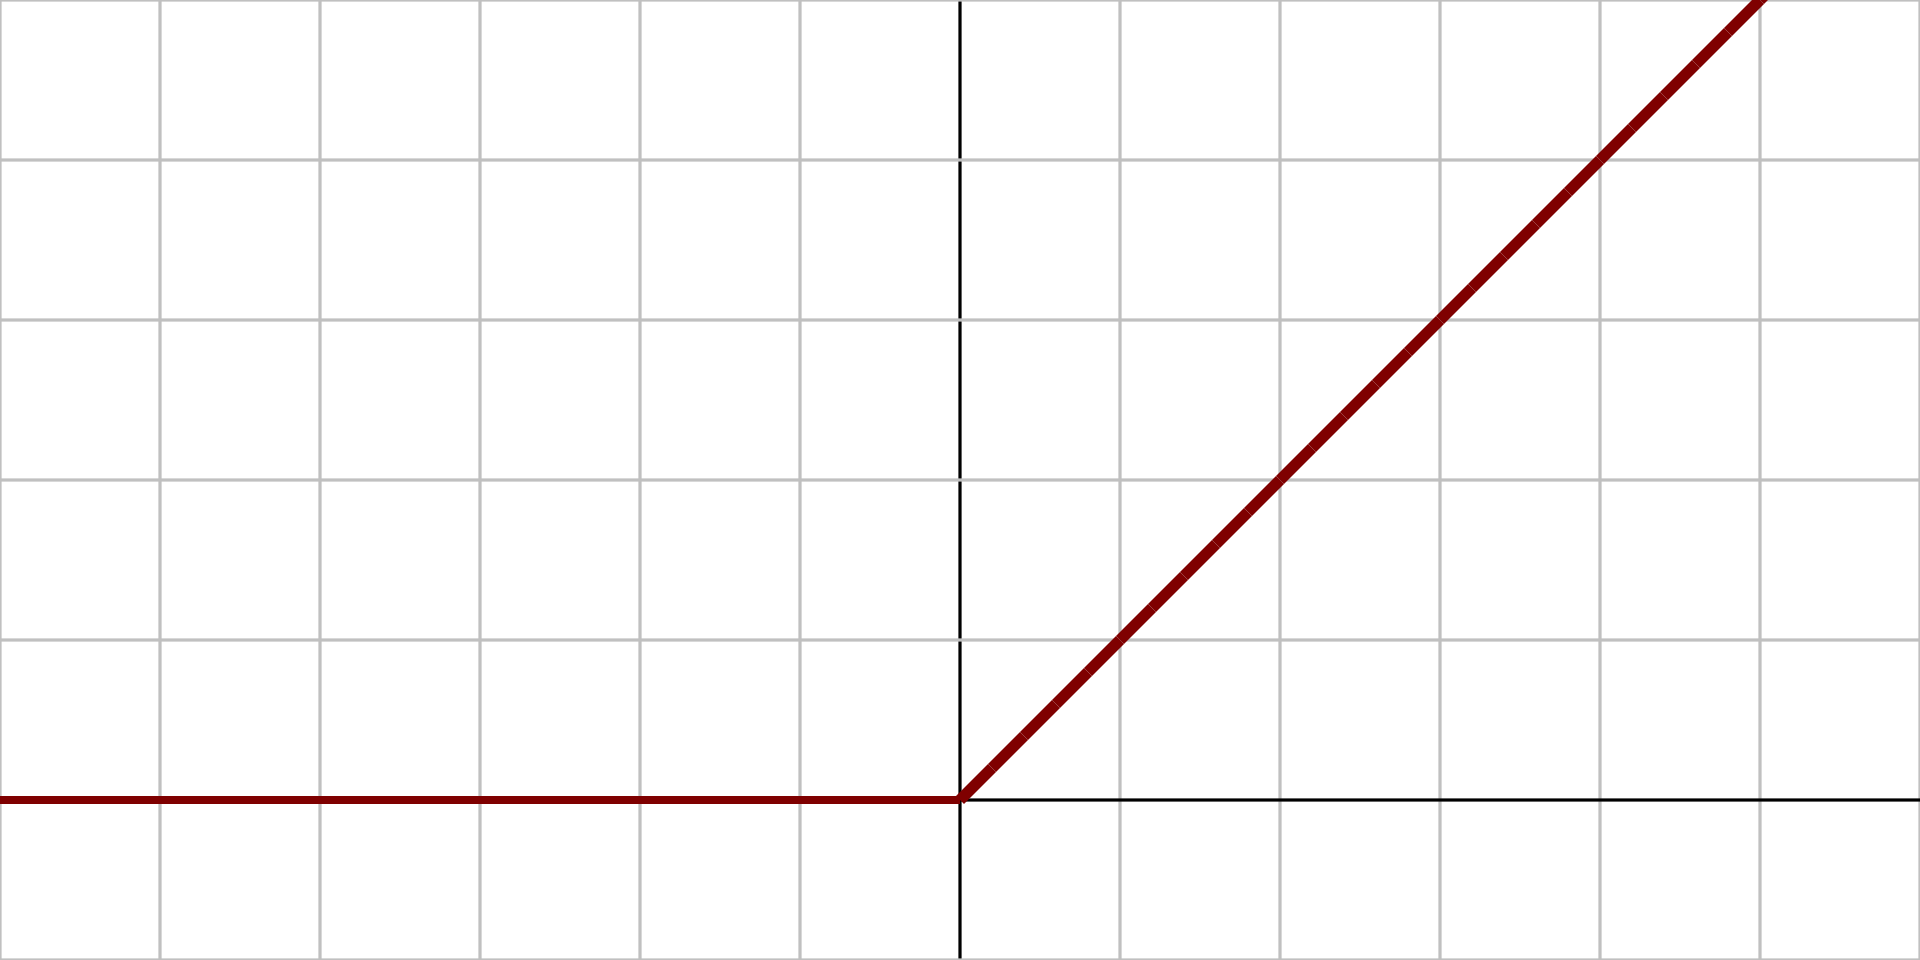
\includegraphics[width=0.5\columnwidth]{figs/Activation_rectified_linear.svg.png}
   \end{center}
   
   \item logistic activation
   \[
   \begin{split}
      &\sigma: \Rbb \mapsto (0;1)\\
      &\sigma(z) = \frac{1}{1 + \e^{-z}}
   \end{split}
   \]
   \begin{center}
   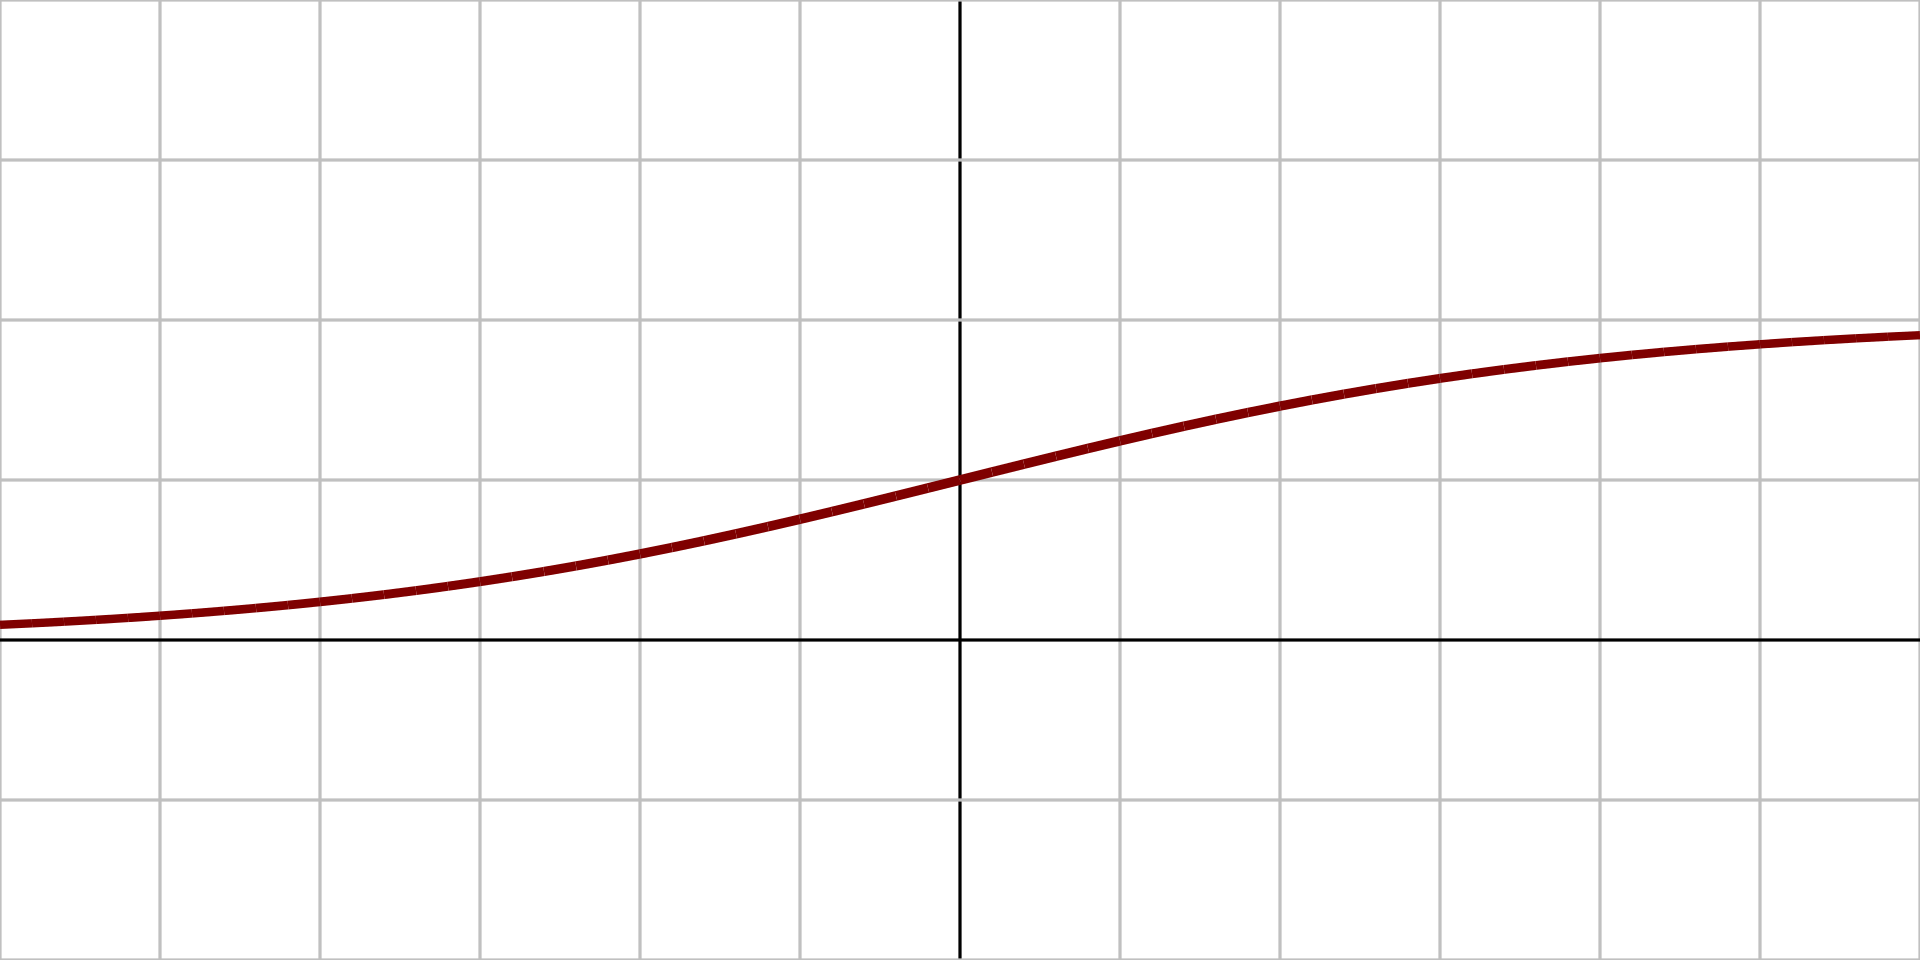
\includegraphics[width=0.5\columnwidth]{figs/Activation_logistic.svg.png}
   \end{center}

   \item hyperbolic tangent activation
   \[
   \begin{split}
      &\tanh: \Rbb \mapsto (-1;+1)\\
      &\tanh(z) = \frac{\e^{z} - \e^{-z}}{\e^{z} + \e^{-z}}
   \end{split}
   \]
   \begin{center}
   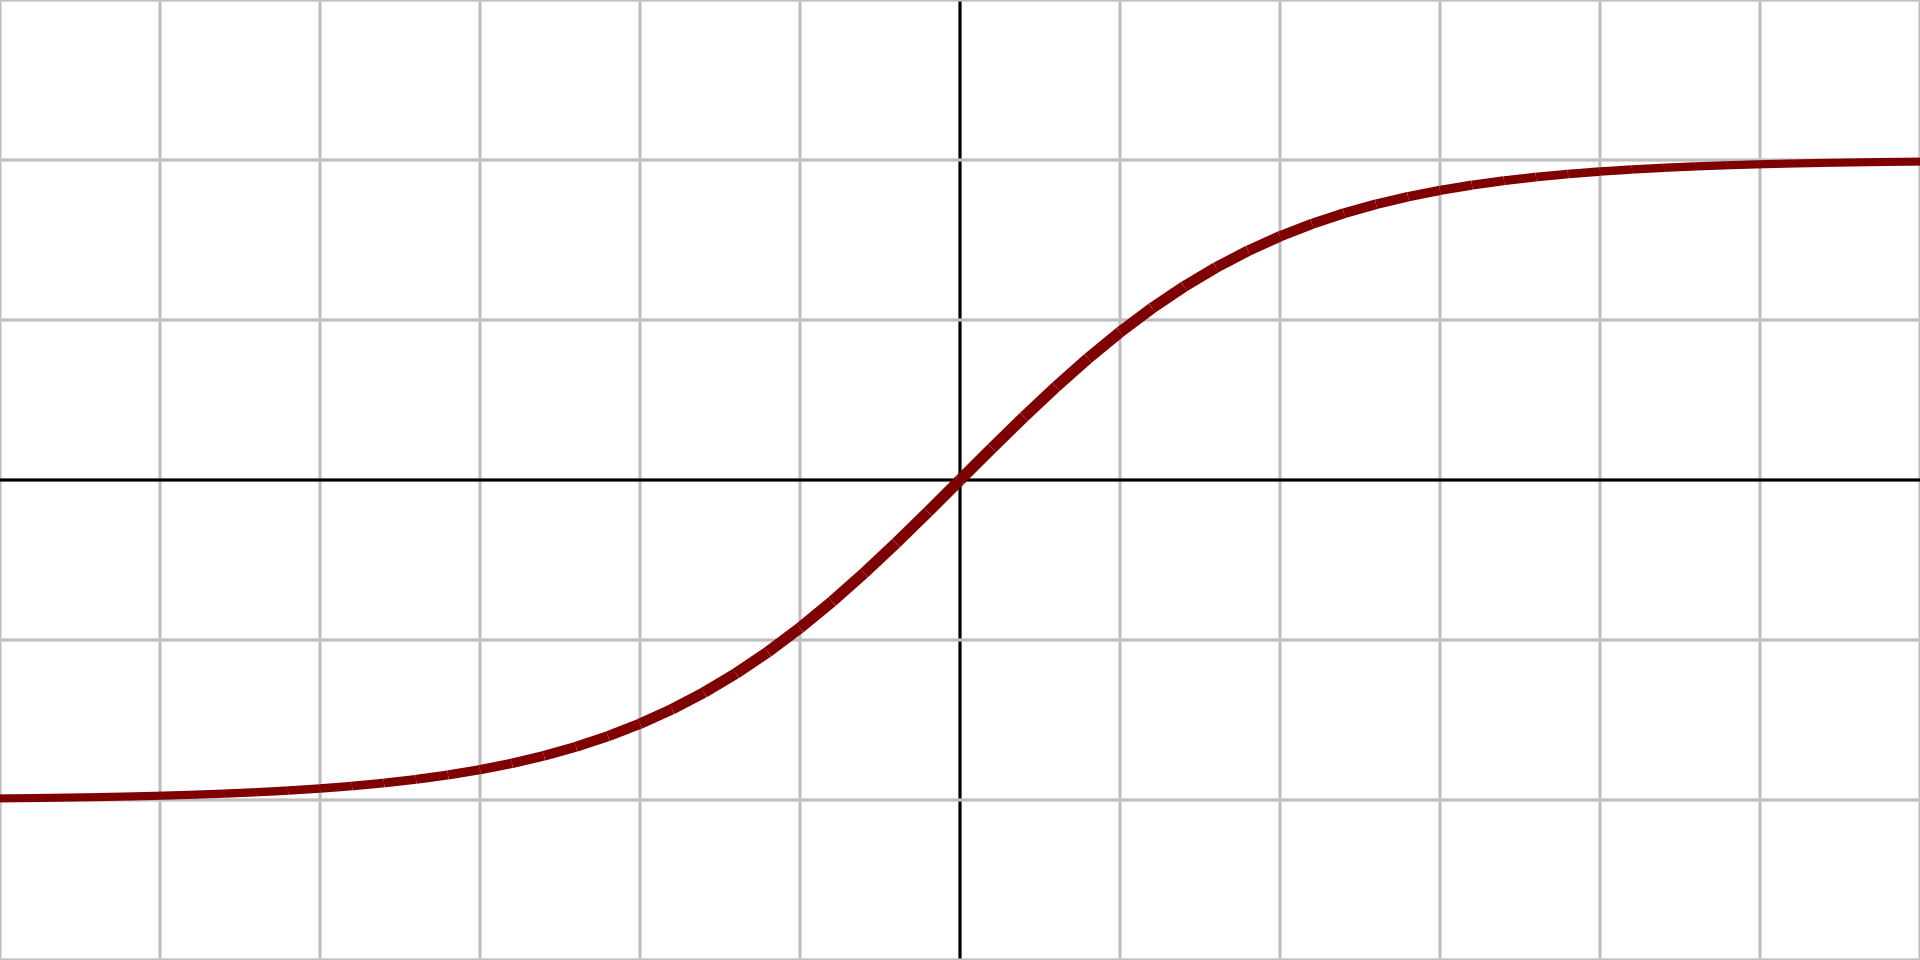
\includegraphics[width=0.5\columnwidth]{figs/Activation_tanh.svg.png}
   \end{center}

   \item Gaussian error linear unit activation
   \[
      \text{GELU}(z) = z \Phi(z)
   \]
   where $\Phi$ is the c.d.f. of the standard normal distribution,
   \begin{center}
   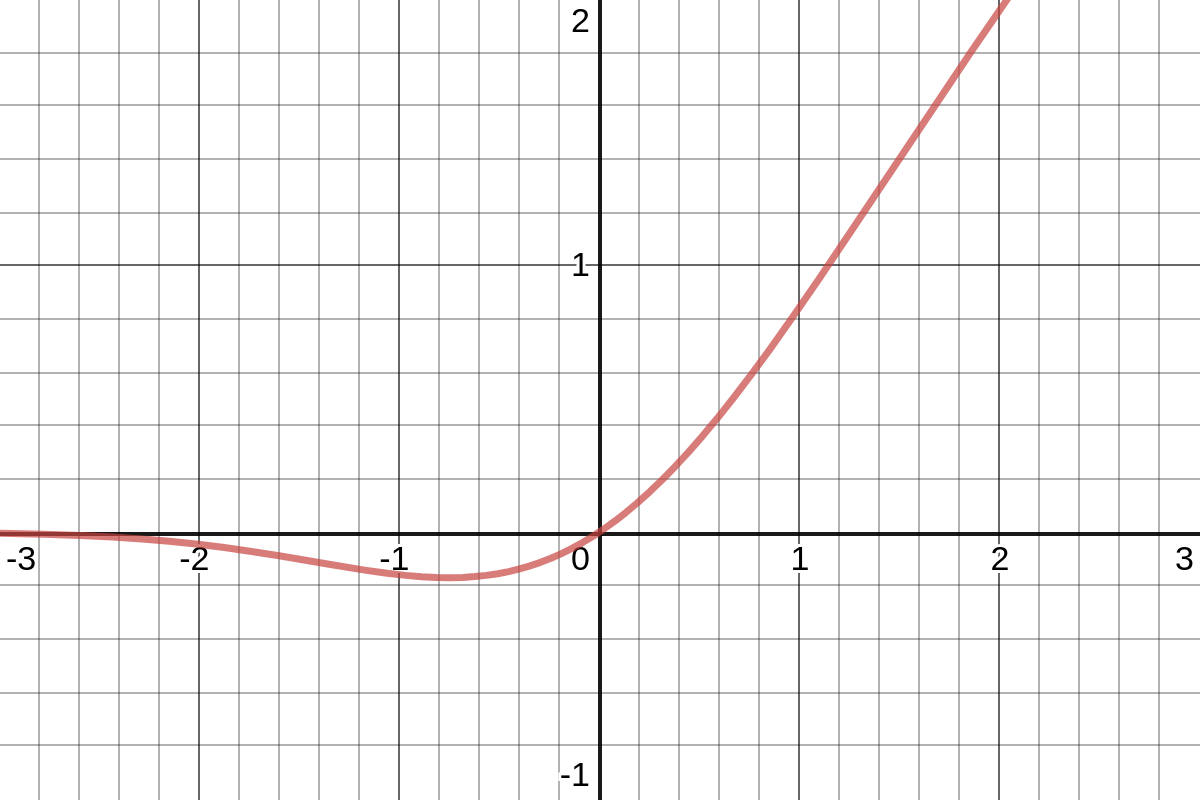
\includegraphics[width=0.5\columnwidth]{figs/Activation_gelu.png}
   \end{center}

   \item sigmoid linear unit activation
   \[
      \text{SiLU}(z) = z \sigma(z)
   \]
   \begin{center}
   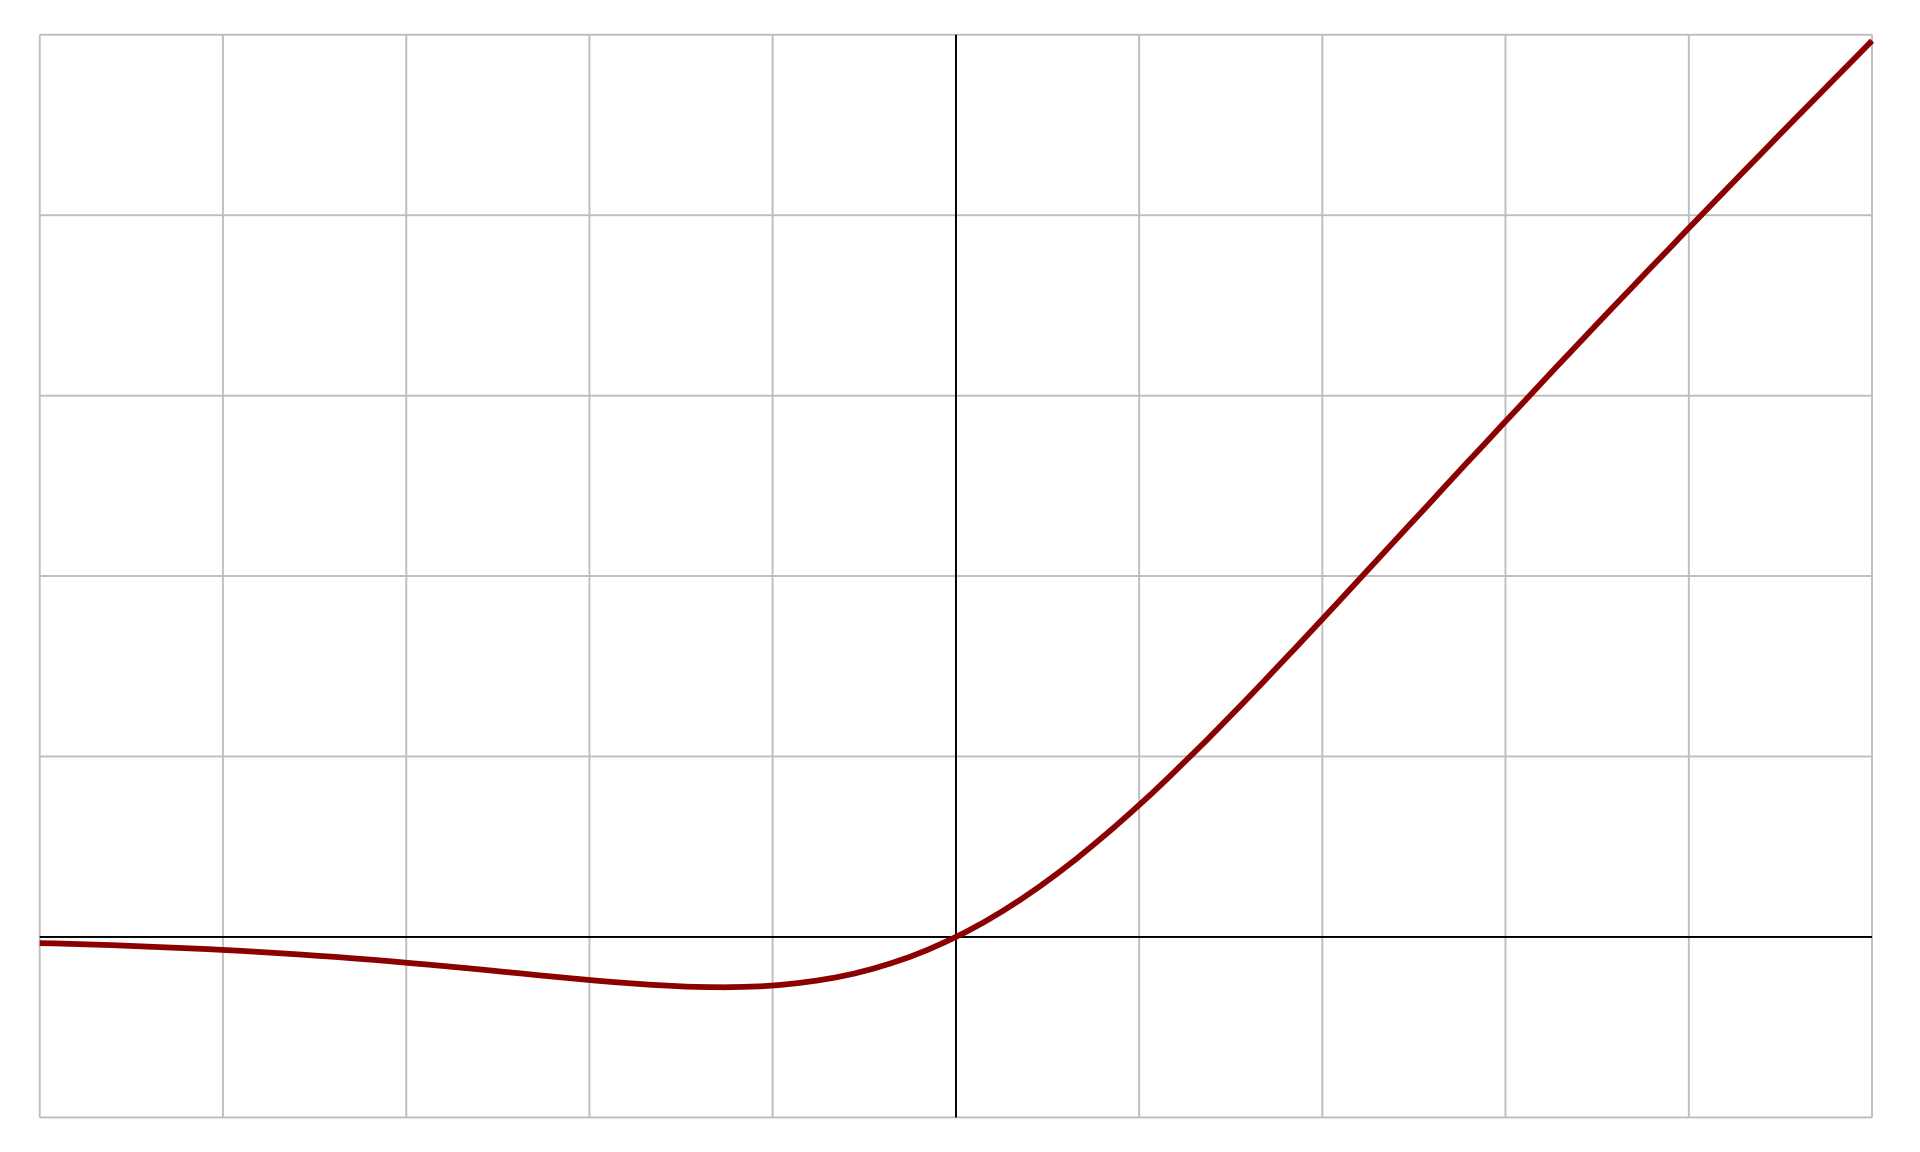
\includegraphics[width=0.5\columnwidth]{figs/Activation_Swish.svg.png}
   \end{center}

\end{itemize}

The first one on the list is the most commonly used activation function, the next two were once very
popular but nowadays find applications only in some specific use-cases, meanwhile the last two are
relatively new modifications of the field-tested ReLU.

Here, we also derive the (very simple) expressions for the vjp-s of both the linear and activation
layers required in the backpropagation algorithm. Indeed for the non-linear activation layer
$\bm{F}$ we have
\[
   \pdv{F_{\alpha'\alpha}}{X_{\mu\nu}} = f'(X_{\alpha'\alpha}) \delta_{\alpha'\mu} \delta_{\alpha\nu}
\]
and thus
\[
\boxed
{
   \pdv{L}{X_{\mu\nu}} = \sum_{\alpha'\alpha} \pdv{L}{F_{\alpha'\alpha}} \pdv{F_{\alpha'\alpha}}{X_{\mu\nu}} = \pdv{L}{F_{\mu\nu}} f'(X_{\mu\nu})\,.
}
\]
On the other hand for the linear layer $\bm{A}$ we have
\[
\begin{split}
   \pdv{A_{\alpha'\alpha}}{X_{\mu\nu}} &= \sum_{\beta} W_{\beta\alpha} \delta_{\alpha'\mu} \delta_{\beta\nu} = W_{\nu\alpha} \delta_{\alpha'\mu}\\
   \pdv{A_{\alpha'\alpha}}{W_{\mu\nu}} &= \sum_{\beta} X_{\alpha'\beta} \delta_{\beta\mu} \delta_{\alpha\nu} = X_{\alpha'\mu} \delta_{\alpha\nu}\\
   \pdv{A_{\alpha'\alpha}}{b_{\mu}   } &= \delta_{\alpha\mu}
\end{split}
\]
and thus
\[
\boxed
{
\begin{split}
   \pdv{L}{X_{\mu\nu}} &= \sum_{\alpha'\alpha} \pdv{L}{A_{\alpha'\alpha}} \pdv{A_{\alpha'\alpha}}{X_{\mu\nu}} = \sum_{\alpha} \pdv{L}{A_{\mu\alpha}} W_{\nu\alpha} \\
   \pdv{L}{W_{\mu\nu}} &= \sum_{\alpha'\alpha} \pdv{L}{A_{\alpha'\alpha}} \pdv{A_{\alpha'\alpha}}{W_{\mu\nu}} = \sum_{\alpha'} \pdv{L}{A_{\alpha'\nu}} X_{\alpha'\mu} \\
   \pdv{L}{b_\mu     } &= \sum_{\alpha'\alpha} \pdv{L}{A_{\alpha'\alpha}} \pdv{A_{\alpha'\alpha}}{b_\mu     } = \sum_{\alpha'} \pdv{L}{A_{\alpha'\mu}}
\end{split}
}
\]

Here, we will also comment on the incorporation of the dropout layers. Note that the dropout layer
$\bm{D}$ is actually just a multiplication of the input tensor by a ''constant'' 0-1 tensor i.e.
\[
   D_{\alpha'\alpha}(\bm{X}) = B_{\alpha'\alpha} X_{\alpha'\alpha}\,.
\]
The tensor $\bm{B}$ is obviously different in the training phase (during which in every forward pass
its every element is randomly sampled from the Bernoulli distribution with given parameter $p$ i.e.
the dropout probability) and the inference phase (during which it is just a constant matrix with
value $p$ being the dropout probability). The vjp-s for the dropout layer required in the
backpropagation algorithm are thus simply given by
\[
\boxed
{
   \pdv{L}{X_{\mu\nu}} = \sum_{\alpha'\alpha} \pdv{L}{D_{\alpha'\alpha}} \pdv{D_{\alpha'\alpha}}{X_{\mu\nu}} = \pdv{L}{D_{\mu\nu}} B_{\mu\nu}\,,
}
\]
where $\bm{B}$ is the current 0-1 matrix sampled in the latest forward pass.


\subsection{RBM}

Generative model is a probabilistic model which enables us to generate new, synthetic observations
similar to the one from training set. Some generative models allow us to estimate the probability
density based on the finite number of samples (observations). There are also generative models in
which we cannot analytically compute the value of the probability density function, however we can
still sample from such model to obtain synthetic observations. Moreover a generative model can
,,explain'' the observations using so called \emph{latent} variables.

We will now focus on the so called \emph{energy based models}. The general idea is to introduce a
parametrized \emph{energy function} \(E(\bm{v},\bm{h}; \bm{\theta})\), where \(\bm{v} \in V
\subseteq \Rbb^{d_v}\) is the observation vector, \(\bm{h} \in H \subseteq \Rbb^{d_h}\) is the
latent variable vector and \(\bm{\theta}\) are the parameters. We now assume that the joint
probability is given by a Boltzmann factor
\[
   p(\bm{v},\bm{h} \mid \bm{\theta}) = \frac{\e^{- E( \bm{v}, \bm{h}; \bm{\theta})}}{Z(\bm{\theta})}
\]
where \(Z(\bm{\theta})\) is the normalization constant
\[
   Z(\bm{\theta}) = \sum_{\bm{v} \in V, \bm{h} \in H} \e^{-E(\bm{v},\bm{h}; \bm{\theta})}
\]
called also (in analogy to statistical physics) -- the \emph{partition function}. Because of the
assumption of the Boltzmann-like probability distribution, these models are often called
\emph{Boltzmann machines}. These models are trained in a similar fashion as standard neural
networks. We first note that given the joint distribution we can compute the marginal distribution
of observations
\[
\begin{split}
   p(\bm{v} \mid \bm{\theta}) &= \sum_{\bm{h} \in H} p(\bm{v},\bm{h} \mid \bm{\theta}) \\
                              &= \frac{1}{Z(\bm{\theta})} \sum_{\bm{h} \in H} \e^{-E(\bm{v},\bm{h}; \bm{\theta})}\,.
\end{split}
\]
and thus can use the standard maximum likelihood criterion to train the model parameters i.e. given
the training set \(\mc{X} = \{\bm{v}^{(1)}, \ldots, \bm{v}^{(N)}\}\) of i.i.d. samples, we seek
parameters \(\bm{\theta}^*\) given by
\[
   \bm{\theta}^* = \argmin_{\bm{\theta}} \left\{ -\frac{1}{N} \sum_{i=1}^N \log p\left(\bm{v}^{(i)} \mid \bm{\theta}\right) \right\}\,.
\]
To find this minimum we will use one of the gradient descent algorithms and thus we will need to
know the derivative of the loss function w.r.t. the parameters. We will now derive the expression
for the derivative for arbitrary energy function. Indeed we have
\[
   \pdv{L(\mc{X}; \bm{\theta})}{\bm{\theta}} = - \frac{1}{N} \sum_{i=1}^N \frac{1}{p\left(\bm{v}^{(i)} \mid \bm{\theta}\right)} \pdv{p\left(\bm{v}^{(i)} \mid \bm{\theta}\right)}{\bm{\theta}}\,.
\]
Expanding the expression for \(p(\bm{v}^{(i)} \mid \bm{\theta})\) we get
\[
\begin{split}
   \pdv{p(\bm{v}^{(i)} \mid \bm{\theta})}{\bm{\theta}} = &- \frac{1}{Z^2(\bm{\theta})} \pdv{Z(\bm{\theta})}{\bm{\theta}} \sum_{\bm{h} \in H} \e^{-E(\bm{v}^{(i)},\bm{h};\bm{\theta})}\\
   &-\frac{1}{Z(\bm{\theta})} \sum_{\bm{h} \in H} \e^{-E(\bm{v}^{(i)},\bm{h};\bm{\theta})} \pdv{E(\bm{v}^{(i)},\bm{h};\bm{\theta})}{\bm{\theta}}
\end{split}
\]
and computing the derivative of partition function we obtain
\[
   \pdv{Z(\bm{\theta})}{\bm{\theta}} = -\sum_{\bm{v} \in V, \bm{h} \in H} \e^{-E(\bm{v},\bm{h};\bm{\theta})} \pdv{E(\bm{v},\bm{h};\bm{\theta})}{\bm{\theta}}
\]
and thus putting it all together we get the following expression for the derivative of loss function
\[
\begin{split}
   &\pdv{L(\mc{X};\bm{\theta})}{\bm{\theta}} \\
   &= -\frac{1}{N} \sum_{i=1}^N \Bigg\{ \sum_{\bm{v} \in V, \bm{h} \in H} \left[ \frac{\e^{-E(\bm{v},\bm{h};\bm{\theta})}}{Z(\bm{\theta})} \cdot \pdv{E(\bm{v},\bm{h};\bm{\theta})}{\bm{\theta}} \right] \\
   &- \sum_{\bm{h} \in H} \left[ \frac{\e^{-E(\bm{v}^{(i)},\bm{h};\bm{\theta})}}{\sum_{\bm{h}' \in H} \e^{-E(\bm{v}^{(i)},\bm{h}';\bm{\theta})}} \cdot \pdv{E(\bm{v}^{(i)},\bm{h};\bm{\theta})}{\bm{\theta}} \right] 
   \Bigg\}
\end{split}
\]
This expression looks awful, but let's notice that
\[
\begin{split}
   p(\bm{h} \mid \bm{v}^{(i)}, \bm{\theta}) &= \frac{p(\bm{v}^{(i)}, \bm{h} \mid \bm{\theta})}{\sum_{\bm{h}' \in H} p(\bm{v}^{(i)}, \bm{h}' \mid \bm{\theta})}\\
                                      &= \frac{\e^{-E(\bm{v}^{(i)},\bm{h};\bm{\theta})}}{\sum_{\bm{h}' \in H} \e^{-E(\bm{v}^{(i)},\bm{h}';\bm{\theta})}}
\end{split}
\]
thus the expression can be written as
\[
\boxed
{
   \begin{split}
      \pdv{L(\mc{X};\bm{\theta})}{\bm{\theta}}= &-\mathbb{E}_{\bm{v},\bm{h} \sim p(\bm{v},\bm{h} \mid \bm{\theta})} \left[ \pdv{E(\bm{v},\bm{h};\bm{\theta})}{\bm{\theta}} \right] \\
      &+ \frac{1}{N} \sum_{i=1}^N \mathbb{E}_{\bm{h} \sim p(\bm{h} \mid \bm{v}^{(i)}, \bm{\theta})} \left[ \pdv{E(\bm{v}^{(i)}, \bm{h}; \bm{\theta})}{\bm{\theta}} \right]
   \end{split}
}
\]
The considerations up until now were quite general. We will now consider a specific Boltzmann
machine called \emph{Restricted Boltzmann Machine}, introduce its' energy function and describe
effective procedures to compute the gradient of the loss function. Restricted Boltzmann machine is an
energy based model with binary units i.e. \(\bm{v} \in V = \{0,1\}^{d_v}\) and \(\bm{h} \in H =
\{0,1\}^{d_h}\), described by the following energy function (for clarity of notation we don't write
the parameters in the energy function arguments)
\[
\begin{split}
   E(\bm{v}, \bm{h}) &= -\bm{v}\bm{b}^\tpose - \bm{h}\bm{c}^\tpose - \bm{v}\bm{W}\bm{h}^\tpose \\
                     &= -\sum_{\alpha} b_\alpha v_\alpha -\sum_{\beta} c_\beta h_\beta - \sum_{\alpha\beta} v_\alpha W_{\alpha\beta} h_\beta
\end{split}
\]
where \(\bm{W}\), \(\bm{b}\), \(\bm{c}\) are the parameters and the vectors are represented as row
matrices. This energy function has a nice property of conditional independence. Indeed consider the
conditional distribution
\[
\begin{split}
   p(\bm{h} \mid \bm{v}) &= \frac{\e^{-E(\bm{v},\bm{h})}}{\sum_{\bm{h}' \in H} \e^{-E(\bm{v}, \bm{h}')}} \\
   &= \frac{\prod_\beta \e^{(c_\beta h_\beta + \sum_\alpha v_\alpha W_{\alpha\beta} h_\beta)}}{ \sum_{\bm{h}' \in H} \prod_\beta \e^{(c_\beta h'_\beta + \sum_\alpha v_\alpha W_{\alpha\beta} h'_\beta)}}
\end{split}
\]
and note that
\[
\begin{split}
   &\sum_{\bm{h}' \in H} \prod_\beta \e^{(c_\beta h'_\beta + \sum_\alpha v_\alpha W_{\alpha\beta} h'_\beta)} \\
   &= \prod_\beta \sum_{h'_\beta \in \{0,1\}} \e^{(c_\beta h'_\beta + \sum_\alpha v_\alpha W_{\alpha\beta} h'_\beta)}
\end{split}
\]
thus
\[
   p(\bm{h} \mid \bm{v}) = \prod_\beta \frac{\e^{(c_\beta h_\beta + \sum_\alpha v_\alpha W_{\alpha\beta} h_\beta)}}{1 + \e^{(c_\beta + \sum_\alpha v_\alpha W_{\alpha\beta})}}
\]
and by symmetry
\[
   p(\bm{v} \mid \bm{h}) = \prod_\alpha \frac{\e^{(b_\alpha v_\alpha + \sum_\beta v_\alpha W_{\alpha\beta} h_\beta)}}{1 + \e^{(b_\alpha + \sum_\beta  W_{\alpha\beta} h_\beta)}}\,.
\]
We can see therefore that given \(\bm{v}\) (or \(\bm{h}\)) each element of \(\bm{h}\) (or \(\bm{v}\))
is given by the Bernoulli distribution with parameters
\[
\begin{split}
   &p(v_\alpha = 1 \mid \bm{h}) = \sigma\left( b_\alpha + \sum_\beta W_{\alpha\beta}h_\beta \right)\\
   &p(h_\beta = 1 \mid \bm{v}) = \sigma\left( c_\beta + \sum_\alpha v_\alpha W_{\alpha\beta} \right)\\
\end{split}
\]
where \(\sigma\) is the logistic function. This observation allows us to compute the second term in
the loss derivative formula
\[
\begin{split}
&\mathbb{E}_{\bm{h} \sim p(\bm{h} \mid \bm{v}^{(i)})}\left[ \pdv{E(\bm{v}^{(i)}, \bm{h})}{W_{\mu\nu}}\right] = -v_\mu^{(i)} \sigma\left(c_\nu + \sum_\alpha v_\alpha^{(i)} W_{\alpha\nu}\right)\\
&\mathbb{E}_{\bm{h} \sim p(\bm{h} \mid \bm{v}^{(i)})}\left[ \pdv{E(\bm{v}^{(i)}, \bm{h})}{b_{\mu}}\right] = -v_\mu^{(i)}\\
&\mathbb{E}_{\bm{h} \sim p(\bm{h} \mid \bm{v}^{(i)})}\left[ \pdv{E(\bm{v}^{(i)}, \bm{h})}{c_\nu}\right] = - \sigma\left(c_\nu + \sum_\alpha v_\alpha^{(i)} W_{\alpha\nu}\right)
\end{split}
\]
The first term however is much more difficult to compute. In fact in practice it is impossible to
compute as it requires summation over exponentially many values. To overcome this problem we
introduce two heuristics which enable us to train RBMs in practice.

\subsubsection{Contrastive Divergence}

The first heuristic is based on a simple observation -- we can estimate the expectation of the
gradient of the energy by sampling \(N\) vectors \(\underline{\bm{v}}^{(i)}\) from marginal
distribution \(p(\bm{v})\) and approximating the true expectation as an average
\[
\begin{split}
   &\mathbb{E}_{\bm{v}, \bm{h} \sim p(\bm{v},\bm{h} \mid \bm{\theta})}\left[\pdv{E(\bm{v},\bm{h}; \bm{\theta})}{\bm{\theta}}\right] \\
   &\approx \frac{1}{N} \sum_{i=1}^N \mathbb{E}_{\bm{h} \sim p(\bm{h} \mid \underline{\bm{v}}^{(i)}, \bm{\theta})}\left[\pdv{E(\underline{\bm{v}}^{(i)},\bm{h}; \bm{\theta})}{\bm{\theta}}\right]\,. 
\end{split}
\]
This is obviously due to the fact that
\[
\begin{split}
   &\mathbb{E}_{\bm{v}, \bm{h} \sim p(\bm{v},\bm{h} \mid \bm{\theta})}\left[ f \right] = \sum_{\bm{v} \in V} \sum_{\bm{h} \in H} f p(\bm{v}, \bm{h} \mid \bm{\theta}) \\
   &= \sum_{\bm{v} \in V} \left\{ \left[ \sum_{\bm{h} \in H} f p(\bm{h} \mid \bm{v}, \bm{\theta}) \right] p(\bm{v} \mid \bm{\theta}) \right\}\\
   &= \sum_{\bm{v} \in V} \mathbb{E}_{\bm{h} \sim p(\bm{h} \mid \bm{v}, \bm{\theta})}[f] p(\bm{v} \mid \bm{\theta})\\
   &\approx \frac{1}{N} \sum_{i=1}^N \mathbb{E}_{\bm{h} \sim p(\bm{h} \mid \underline{\bm{v}}^{(i)}, \bm{\theta})}[f]
\end{split}\quad.
\]
Since we can easily compute the conditional expectation, using the above formula we can estimate the
true gradient of the parameters. How do we sample from the marginal distribution distribution? We
can use the Gibbs sampling algorithm which is an instance of general class of MCMC (Markov Chain
Monte Carlo) algorithms. We start with \(\underline{\bm{v}}_0^{(i)} = \bm{v}^{(i)}\), next we sample
\(\underline{\bm{h}}_1^{(i)}\) from the conditional distribution \(p(\bm{h} \mid
\underline{\bm{v}}_0^{(i)})\), after that we sample \(\underline{\bm{v}}_1^{(i)}\) from \(p(\bm{v}
\mid \underline{\bm{h}}_1^{(i)})\) and so on. We repeat the steps \(k\) times and in the end obtain
samples \(\underline{\bm{v}}_k^{(i)}\). We then approximate the expectations as
\[
\begin{split}
&\mathbb{E}_{\bm{v},\bm{h} \sim p(\bm{v},\bm{h})}\left[ \pdv{E(\bm{v}, \bm{h})}{W_{\mu\nu}}\right] \approx - \frac{1}{N}\sum_{i=1}^N \underline{v}_\mu^{(i,k)} \sigma\left(c_\nu + \sum_\alpha \underline{v}_\alpha^{(i,k)} W_{\alpha\nu}\right)\\
&\mathbb{E}_{\bm{v},\bm{h} \sim p(\bm{v},\bm{h})}\left[ \pdv{E(\bm{v}, \bm{h})}{b_{\mu}}\right] \approx - \frac{1}{N}\sum_{i=1}^N \underline{v}_\mu^{(i,k)}\\
&\mathbb{E}_{\bm{v},\bm{h} \sim p(\bm{v},\bm{h})}\left[ \pdv{E(\bm{v}, \bm{h})}{c_\nu}\right] \approx - \frac{1}{N}\sum_{i=1}^N \sigma\left(c_\nu + \sum_\alpha \underline{v}_\alpha^{(i,k)} W_{\alpha\nu}\right)
\end{split}
\]
and are finally able to compute the gradients and update the parameters.


\subsubsection{Persistent Contrastive Divergence}

The algorithm described in the previous paragraph has one serious flaw -- it is extremely slow, as
for it to work properly each parameters' update would require hundreds or thousands of Gibbs
sampling steps. In practice it is, therefore, often implemented in such a way that we only perform
few sampling steps (even as few as 1) but this comes with a serious problem -- we no longer
approximate the true expectation with random error -- the error is now systematic.

To overcome this difficulty we introduce the idea of a \emph{persistent chain}. The core idea is to
spread the Gibbs sampling computation over many parameters' updates, i.e. during each parameters'
update we perform only a few Gibbs sampling steps but retain the set of hidden vectors
\(\bm{h}^{(j)}\) (which we will call the persistent chain) from which we start sampling in the next
update. The outline of the algorithm is thus as follows -- first we initialize the persistent chain
\(\{\bm{p}^{(j)} = \bm{0}\}_{j=1}^M\); during each parameters' update we perform \(k\) Gibbs
sampling steps starting from \(\underline{\bm{h}}_1^{(j)} = \bm{p}^{(j)}\) and obtain a sample
\(\bm{v}_k^{(j)}\), we approximate the expectations as before (noting that now we average over \(M\)
samples) and in the end update the persistent chain by sampling \(M\) vectors \(\bm{p}^{(j)}\) from
the distribution \(p(\bm{h} \mid \underline{\bm{v}}_k^{(j)})\).


\subsection{DBN}

Let's note that RBM can be interpreted as a network of units connected in layers as depicted in the
figure below. The nodes on the left represent the visible binary units, the nodes on the right
represent the hidden units and edges represent the interactions of the type \(W_{\alpha\beta}
v_\alpha h _\beta\) (there are also biases, not depicted in the picture).

\begin{figure}[ht]
   \centering
   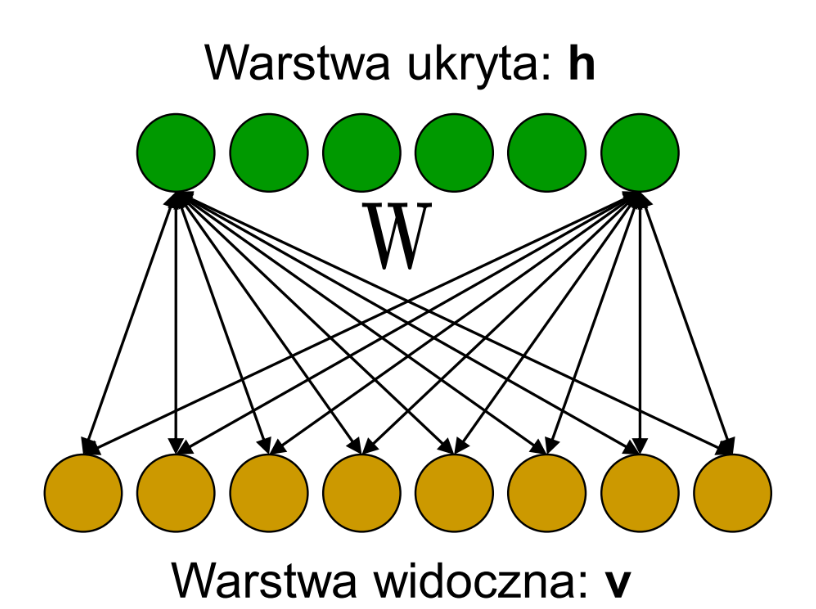
\includegraphics[width=0.65\columnwidth]{figs/rbm.png}
   \label{fig:rbm}
   \caption{Schematic depiction of RBM with 8 visible units and 6 hidden units}
\end{figure}

Note that before we had not made any explicit connection between the RBM and neural networks. We
simply treated it like an energy based model and the energy function was our primary object of
interest. The interpretation of the RBM as an undirected, stochastic neural network is possible only
due to the conditional independence property of $p(\bm{h} \mid \bm{v})$ and $p(\bm{v} \mid \bm{h})$.
The network thus operates as follows -- we feed it some binary example vector $\bm{v}$, then compute
the \emph{activations} of the hidden units $\sigma(\bm{b} + \bm{v}\bm{W})$ and then sample the
hidden units given the activations from the Bernoulli distributions, we can then do the same thing
in the opposite direction and sample from the visible layer. Performing these steps many times (that
is performing Gibbs sampling) we obtain in the end an artificial sample from the network itself and
if the network has been trained on some data $\mc{X}$ then these samples are similar (but not the
same) to the empirical samples.

Deep Belief Network (DBN) is basically multiple RBMs stacked on top of each other as depicted in the
picture below. We can implement this network as a sequence of RBMs with parameters $\bm{W}^{(1)},
\bm{b}^{(1)}, \bm{c}^{(1)}$, $\ldots$, $\bm{W}^{(l)}, \bm{b}^{(l)}, \bm{c}^{(l)}$ respectively ($l$
being the number of layers). We can train the DBN using a simple heuristic called \emph{greedy
layer-wise training}. The idea is simple -- we sequentially train each RBM $i$ on the dataset
$\mc{X}$ propagated through the $i-1$ first layers (i.e. we compute only the activations and do not
sample the units -- this still turns out to be working but slightly differs from the theory
presented above). After training we can sample DBN by propagating the visible units $\bm{v}$ up to
the last RBM, performing Gibbs sampling in this last RBM and propagating the output down to the
first RBM.

\begin{figure}[ht]
   \centering
   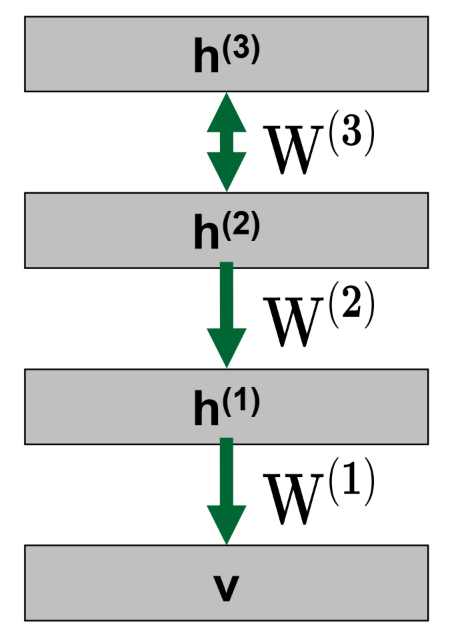
\includegraphics[width=0.45\columnwidth]{figs/dbn.png}
   \label{fig:dbn}
   \caption{Schematic depiction of DBN with 4 layers}
\end{figure}


\subsubsection{MLP initialization using DBN}

DBNs can be used to initialize weights in the MLP layers and thus improve the overall performance of
the MLP network. The improvement can be huge, especially if we have lots of unlabeled data and only
a handful of labeled examples as is the case e.g. when the labeling process is costly, difficult or
time-consuming. The implementation is straight-forward. We train the $n$-layer-deep DBN in an
unsupervised manner using the greedy layer-wise training algorithm. We then construct an MLP with
$n+1$ layers, initialize the first $n$ layers with the weights and biases of the pretrained DBN and
finetune the MLP on the smaller set of labeled examples. This type of initialization is also called
\emph{greedy layer-wise pretraining}. One key aspect to remember when using this approach is that
the activations of the MLP must match the ''activations'' of the DBN. If we use the logistic sigmoid
activations in the MLP then nothing is changed in the RBM, however if we would like to use ReLU
activation function then one may show that the RBM activations should given by $\text{ReLU}(\bm{b} +
\bm{vW})$ and to sample the hidden units we should use the so called \emph{noisy rectified linear
unit} 
\[
   \text{N-ReLU}(z) = \max\{ 0, z + \sqrt{\sigma(z)} \cdot \epsilon\}\,,
\]
where $\epsilon \sim \mc{N}(0,1)$.


\subsection{Autoencoder}

Autoencoder is a general type of neural architecture used for unsupervised learning. The idea is to
construct two networks: an encoder network and a decoder network and connect them through the so
called \emph{bottleneck layer}. The encoder, given some high-dimensional input data, compresses them
into much more compact representation and the decoder can reconstruct the original data from this
compact representation. The encoder and the decoder are trained jointly and learn the suitable
representations together. If we care only about the learnt representations we can discard the
decoder after training and use only the encoder part.

\begin{figure}[ht]
   \centering
   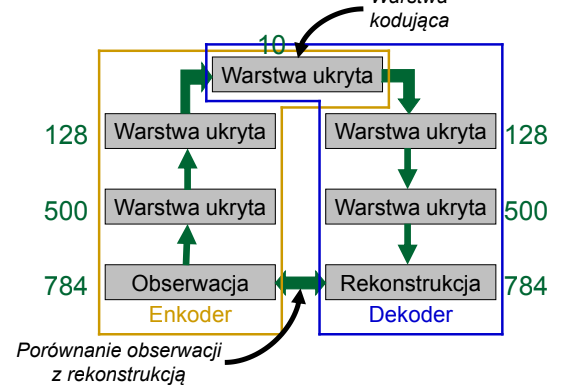
\includegraphics[width=0.95\columnwidth]{figs/autoencoder.png}
   \label{fig:ae}
   \caption{Schematic depiction of a general autoencoder architecture}
\end{figure}

One important aspect of the training process of the autoencoder is the choice of the loss functions.
Since the output of the autoencoder should be as close as possible to the input the typical choice
would be the L2 loss. If the data can be modelled using sigmoid units then perhaps the pixelwise
cross-entropy loss would be more suitable.

\subsection{CNN}

Convolutional neural network (CNN) is a type of neural architecture adapted to processing data with
certain spatial interdependencies. An obvious example of such data are images represented as
3-dimensional arrays $X_{c,x,y}$ where the 1st dimension is the so called ''channel'' dimension (R,
G, B) and the other two dimension contain the pixel intensities of the given channel. Processing
such data using basic fully-connected networks would be incredibly inefficient as the number of
weights would basically scale quadratically with the number of pixels. Convolutional and pooling
layers which form the basic building blocks of a CNN were designed to remedy this problem.
\[
\boxed{
\begin{split}
   &\text{Conv2D}_{\beta,c,x,y}(\bm{X}; \bm{K}, \bm{b}) = \\
   & b_c + \sum_{c'=0}^{C_\text{in}-1} \sum_{x'=0}^{H_\text{filter}-1} \sum_{y'=0}^{W_\text{filter}-1} X_{\beta, c', d_x x' + s_x x, d_y y' + s_y y} \cdot K_{c,c',x',y'}   
\end{split}
}
\]
The input to the layer is a stack (batch) of $B$ 3-dimensional tensors with shapes $(C_\text{in},
H_\text{in}, W_\text{in})$ each. The set of the layer's parameters consists of a vector $\bm{b}$ of
shape $(C_\text{out},)$ and a stack $\bm{K}$ of $C_\text{out}$ 3-dimensional \emph{filters} (or
\emph{kernels}) of shape $(C_\text{in}, H_\text{filter}, W_\text{filter})$ each. Additionally the
layer has specified hyperparameters: $s_x$, $s_y$ (\emph{strides}), $d_x$, $d_y$ (\emph{dilations}).
The output of the layer is a batch of $B$ 3-dimensional tensors with shapes $(C_\text{out},
H_\text{out}, W_\text{out})$ where
\[
\boxed{
\begin{split}
   H_\text{out} =& \left\lfloor \frac{H_\text{in} - d_x \cdot (H_\text{filter} - 1) - 1}{s_x} + 1 \right\rfloor \\
   W_\text{out} =& \left\lfloor \frac{W_\text{in} - d_y \cdot (W_\text{filter} - 1) - 1}{s_y} + 1 \right\rfloor \\
\end{split}
}
\]
\begin{figure}[ht]
   \centering
   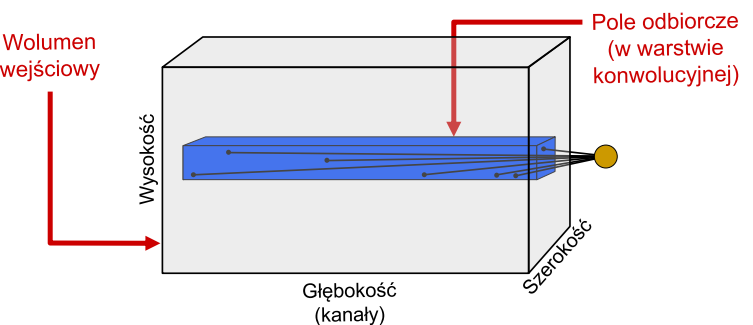
\includegraphics[width=0.9\columnwidth]{figs/conv2d.png}
   \label{fig:conv2d}
   \caption{Schematic representation of a convolution operation}
\end{figure}

Let's note here an important property of the convolutional layer -- it is \emph{equivariant} to
translations of the object in the picture. Indeed the translation of the object corresponds to the
equivalent translation of the activations of the layer. The whole network (after applying many
convolutional layers, flattening and softmax) shoud thus be \emph{invariant} to such translations.
Convolutional architecture has therefore a baked-in bias suitable for image data. The convolutional
layer changes both the channel dimension and height / width. We can also use padding to counter the
height / width shrinkage. 

Pooling layers on the other hand are parameter-free layers that operate on each input channel
independently and thus do not change the channel dimension but reduce the height / width of the
input. Typically we use max-pooling which for a receptive field returns the maximum pixel value.

\begin{figure}[ht]
   \centering
   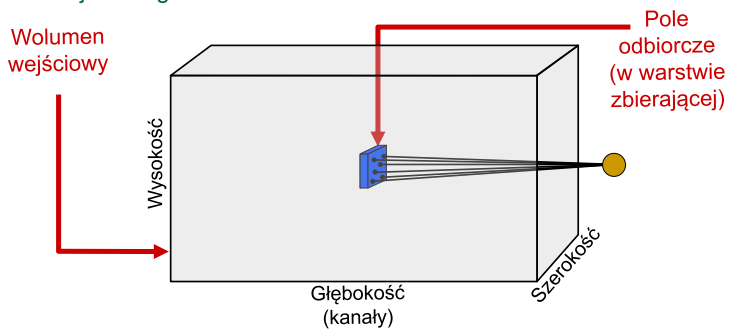
\includegraphics[width=0.9\columnwidth]{figs/maxpool.png}
   \label{fig:pool}
   \caption{Schematic representation of a pooling operation}
\end{figure}

\subsubsection{Residual connections}

Empirical studies of the VGG (Visual Geometry Group) CNNs showed that increasing the depth of the
network improved accuracy up to a certain point, beyond which the performance deteriorated. One
possible heuristic used to prevent this effect was the introduction of residual connections. This
trick is based on an empirical observation that given some complex, nonlinear transformation
$\bm{f}(\bm{x})$ it is often easier to model and learn the residual transformation i.e.
$\bm{f}(\bm{x}) - \bm{x}$. The idea is thus to add special connections between layers of the network
so that the parametrized layers learn this residual transformation which is then added to the input
to model the full transformation as shown in the Figure \ref{fig:residual}.

\begin{figure}[ht]
   \centering
   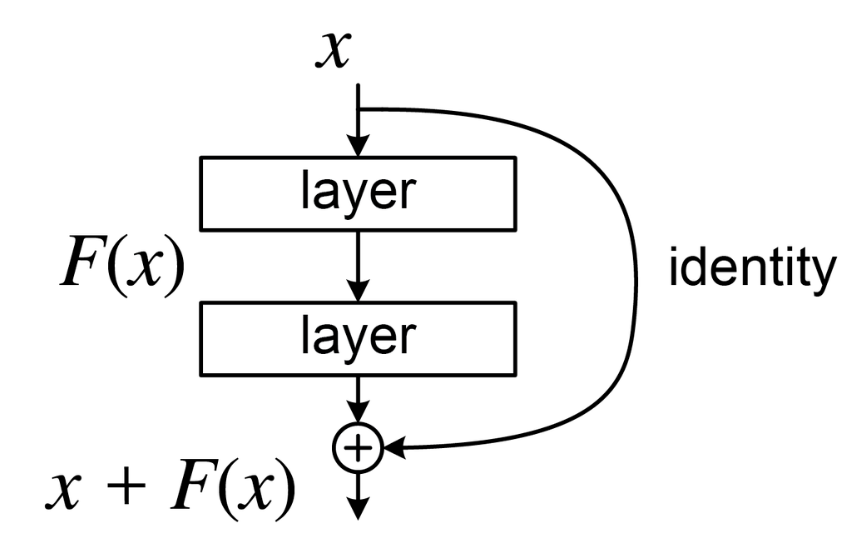
\includegraphics[width=0.75\columnwidth]{figs/residual.png}
   \label{fig:residual}
   \caption{Schematic representation of a residual connection}
\end{figure}

Of course the output of the series of layers must have compatible shape. We can note that such
mechanism certainly improves the gradients flow through the network which might be one of the
reasons for its success.

\subsubsection{Some implementation details}




\end{document}

% TODO:
% * Architecture
%   - GAN
%   - Transformer
%   - ?other?
% * ?CV?
% * ?NLP?
